\documentclass[article]{aaltoseries}
\usepackage[utf8]{inputenc}


\begin{document}
 
%=========================================================

\title{Title of the seminar paper}

\author{Teemu Teekkari% Your first and last name: do _not_ add your student number
\\\textnormal{\texttt{teemu.teekkari@aalto.fi}}} % Your Aalto e-mail address

\affiliation{\textbf{Tutor}: Some Researcher} % First and last name of your tutor

\maketitle

%==========================================================

\begin{abstract}
  This LaTeX template is used for typesetting
  the seminar papers for the Seminar in Computer Science.

\vspace{3mm}
\noindent KEYWORDS: keywords, separated by commas

\end{abstract}


%============================================================


\section{Introduction}

To be added.


%============================================================


\section{Simple things first}

In this section, we give some simple examples of Latex mark-up.
Sec.~\ref{sec:emphasis} emphasizes important points and
Sec.~\ref{sec:math} gives examples of math formulas.
Finally, \ref{sec:list} demonstrates lists.


%------------------------------------------------------------


\subsection{Emphasizing text}
\label{sec:emphasis}

\textit{Italics} is a good way to emphasize printed text. However,
\textbf{boldface} looks better when converted to HTML.

Paragraphs are separated by an empty line in the Latex source code.
Latex puts extra space between sentences, which you must suppress
after a period that does not end a sentence, e.g.\ after this acronym.

Cross-references to figures (Fig.~\ref{fig:mypicture1}), tables
(Table~\ref{tab:mytable1}), other sections (Sec.~\ref{sec:math})
are easy to create. 


%------------------------------------------------------------


\subsection{Mathematics}
\label{sec:math}

In the mathematics mode, you can have subscripts such as $K_{master}$
and superscripts like $2^x$. Longer formulas may be put on a separate
line:
\[ \emptyset \in \emptyset \; \Rightarrow \; E \neq mc^2. \]

You may also want to number the formulas like Eq.~(\ref{eqn:myequation1})
below.
\begin{equation}\label{eqn:myequation1}
C = E_{K_{public}}(P) = P^e. \hspace{10mm}   P = D_{K_{private}}(C) = C^d.
\end{equation}



%------------------------------------------------------------


\subsection{Make a list}
\label{sec:list}

Lists can have either bullets or numbers on them. 

\begin{itemize}
\item one item
\item another item, which is an exceptionally long one for an item
  and consequently continues on the next line.
\end{itemize}

Lists can have several levels. Item~\ref{kukkuu} below contains
another list.
\begin{enumerate}
\item the fist item \label{kukkuu}
  \begin{enumerate}
  \item the first subitem 
  \item the second subitem
  \end{enumerate}
\item the second item
\end{enumerate}


%============================================================


\section{More complex stuff}

This section provides examples of more complex things.


%------------------------------------------------------------


\subsection{Data served on a table}


Table~\ref{tab:mytable1} presents some data in tabular form. 

\begin{table}[t!]
  \begin{center}
    \begin{tabular}{|l|lr|}
    \hline
    Protocol & Year &  RFC \\
    \hline
    TCP      & 1981 &  793 \\
    ISAKMP   & 1998 & 2408 \\
    Photuris & 1999 & 2522 \\
    \hline
    \end{tabular}
    \caption{A table with some protocols}
    \label{tab:mytable1}
  \end{center}
\end{table}


%------------------------------------------------------------


\subsection{Adding references}
\label{sec:references}

Do not forget to give pointers to the literature. If you are listing
stuff related to your topic, you can give several references once
\cite{Com00,HTS03,Nik99}. However, usually you should give only one, for example the standard describing the stuff \cite{RFC2408} and if you want to directly use someone else's words, use both quotation marks and refer to the source, for example that ``the developer does not need to know all about the framework to develop a working implementation'' \cite{Suo98}. Remember also to mark references to your pictures if they are not created by your own mind!

If you plan to write with Latex regularly, create your own BibTeX
database and use BibTeX to typeset the bibliographies automatically.
In the long run, it will save you a lot of time and effort compared to
compiling reference lists by hand.


%------------------------------------------------------------


\subsection{Embedded pictures}
\label{sec:pictures}

Fig.~\ref{fig:mypicture1} is an embedded picture. The supported formats for pictures
depend on the actual LaTeX command used. For instance, regular \LaTeX supports
pictures in EPS (Embedded PostScript) format, while pdf\LaTeX supports PDF (Portable
Document Format), PNG (Portable Network Graphics) and JPEG (Joint Photographic Experts
Group). It is recommended to use either EPS or PDF for diagrams as well as for any picture
which includes vector images.

\begin{figure}[t!]
  \begin{center}
    % Note how the file extension has been removed from the filename below
    % so that the LaTeX command can automatically pick any supported file format
    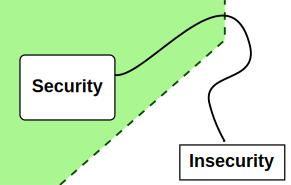
\includegraphics[width=.5\textwidth]{figures/sample}
    \caption{An embedded picture}
    \label{fig:mypicture1}
  \end{center}
\end{figure}


%============================================================


\section{Yet another section title}

To be added.


%============================================================


\section{Conclusion}

To be added.


%============================================================


\bibliographystyle{plain}
\bibliography{cs-seminar}

\end{document}
